% The MIT License (MIT)
%
% Copyright (c) 2021 Polystat.org
%
% Permission is hereby granted, free of charge, to any person obtaining a copy
% of this software and associated documentation files (the "Software"), to deal
% in the Software without restriction, including without limitation the rights
% to use, copy, modify, merge, publish, distribute, sublicense, and/or sell
% copies of the Software, and to permit persons to whom the Software is
% furnished to do so, subject to the following conditions:
%
% The above copyright notice and this permission notice shall be included
% in all copies or substantial portions of the Software.
%
% THE SOFTWARE IS PROVIDED "AS IS", WITHOUT WARRANTY OF ANY KIND, EXPRESS OR
% IMPLIED, INCLUDING BUT NOT LIMITED TO THE WARRANTIES OF MERCHANTABILITY,
% FITNESS FOR A PARTICULAR PURPOSE AND NON-INFRINGEMENT. IN NO EVENT SHALL THE
% AUTHORS OR COPYRIGHT HOLDERS BE LIABLE FOR ANY CLAIM, DAMAGES OR OTHER
% LIABILITY, WHETHER IN AN ACTION OF CONTRACT, TORT OR OTHERWISE, ARISING FROM,
% OUT OF OR IN CONNECTION WITH THE SOFTWARE OR THE USE OR OTHER DEALINGS IN THE
% SOFTWARE.

\documentclass[nosecurity,nobrand]{huawei}
\usepackage{ffcode}
\usepackage{href-ul}
\renewcommand*\theauthor{Yegor Bugayenko}
\renewcommand*\thecompany{Polystat.org}
\renewcommand*\thetitle{{\scshape Polystat}: New Object Calculus\\to Improve Static Program Analysis}
\addbibresource{main.bib}

\newcounter{sector}[section]
\renewcommand\thesector{\thesection.\arabic{sector}}
\newcommand{\sector}[1]{\refstepcounter{sector}\vspace{6pt}\textbf{\textsc{\thesector $\;$ #1}}\quad}

\usetikzlibrary{positioning}
\usetikzlibrary{shapes}
\usetikzlibrary{shapes.multipart}
\usetikzlibrary{arrows}
\usetikzlibrary{arrows.meta}
\usetikzlibrary{fit}
\tikzset{
  every node/.append style={thick, font=\sffamily},
  every path/.append style={thick, draw=black},
  every edge/.append style={every node/.style={font=\sffamily\scriptsize, draw=black, fill=white}},
  every text node part/.append style={align=center}
}
\tikzstyle{arrow} = [-{Latex[width=3mm]}]
\newcommand\component[4][]{
  % #1 (optional) - Additional style for the node
  % #2 - Tikz name
  % #3 - Location
  % #4 - Body
  % for example: \component{farm}{2,2}{Farm}
  \node [outer sep=1mm] at (#3) (#2) {
    \tikz {
      \node[draw=black, fill=white, thick, inner sep=24pt, #1] (r) {\large\texttt{#4}};
      \node[anchor=north east, outer sep=2pt] at (r.north east) {
        \tikz {
          \draw[thick, draw=black] (0,0) rectangle +(0.5,0.5);
          \draw[thick, draw=black, fill=white] (-0.15,0.1) rectangle +(0.3,0.1);
          \draw[thick, draw=black, fill=white] (-0.15,0.3) rectangle +(0.3,0.1);
        }
      }
    }
  };
}

\begin{document}

\maketitle

The quality of software, as one of the most important factors of business success in modern economy,
may be increased by using static program analysis.
The majority of modern programs are written in object-oriented programming languages,
like Java or C++, while most static analysis methods treat them as procedural and
algorithmic ones, reducing the ability to better understand programmers' intent and find
more functional defects. The absence of a formal object calculus
behind modern object-oriented languages is one of the key reasons.
A development of such a calculus and using it in static analysis may
significantly contribute to object-oriented programming as a whole and
move static analysis to a principally new level.

\section{Background}

\sector{What Is Static Analysis?}
As was studied by~\citet{planning2002economic},
software bugs costed the U.S. economy about \$59.5 billion annually.
Static program analysis is a valuable part of software quality control
and is performed without actually executing programs, as explained
by~\citet{wagner2005comparing} and~\citet{moller2012static}.
A growing commercial use of static analysis is in the verification of
properties of software used in safety-critical computer systems and
locating potentially vulnerable code, as noted by~\citet{chess2007secure}.
According to~\citet{jackson2000software},
the importance of code analysis of all kinds will only grow in the future.

\sector{Usefulness}
Static analyzers suggest programmers to pay attention
to certain locations in the source or binary code, highlight good candidates
for fixing, and sometimes even suggest fixes.
The final decision of whether to fix the code or
leave it ``as is''
is made by the programmer. Very often the code is delivered to end-users
without fixing the bugs found by analyzers, as noted by~\citet{steidl2014prioritizing}.
Also, as shown by~\citet{kremenek2003z}, most warnings do not indicate real bugs.
However, according to~\citet{sadowski2018lessons},
only a few percent of programmers react negatively to recommendations of analyzers.

\sector{Unsoundness}
Some functional bugs may be mistakenly reported where the code
is actually correct or couldn't have led to significant misbehavior of the
software~\citep{wagner2005comparing}. Moreover, big proportion of ``false positive''
results in static analysis tools being disregarded by developers as was examined
by~\citet{johnson2013don}. The inaccuracy due to ``false positives'' is known as
``unsoundness'' of analysis~\citep{jackson2000software}.
It was explained by~\citet{moller2012static} that ``a program analyzer is
sound if it never gives incorrect results (but it may answer \emph{maybe}).''
Accuracy of 70\% is considered to be high
for modern analyzers, since ones that effectively find errors have ``false positive''
rates from 30\% to 100\%~\citep{engler2000checking, foster2002flow, 10.1145/349299.349328, wagner2000first}.
As noted by~\citet{gosain2015static}, ``precise analysis is more costly.''

\sector{Standards}
There are organizations, such as MISRA, SEI, MITRE and ISO, which publish
guidelines, recommendations and standards
for software developers~\citep{misra2012,cert2016,iso26262,do178c,iec62304,iec62279,iec61508}.
Some static analyzers take those recommendations into account and get
certified, for example,
Coverity, Klocwork and CodeSonar are such analyzers certified by T\"uV S\"uD.

\sector{Front-End}
Most analyzers have three major components of their architecture,
as described by~\citet{binkley2007source}:
the parser, the internal representation, and the analysis of this representation.
The parser, which usually includes lexer, preprocessor, and tokenizer (together known as ``front-end'')
in most analyzers is language-specific: it can only parse a source
code written in one or a few programming languages. Some analyzers are polyglots,
which usually is realized via an intermediary language (also known as ``intermediary representation'' or IR),
which the source language is translated into, before the analysis is done. For example,
Phasar~\citep{phasar}, CodeChecker~\citep{codechecker} and Clang Static Analyzer~\citep{clang}
are open source analyzers of such kind---they
analyze LLVM code~\citep{lattner2004llvm},
which may be generated from C/C++, Java, C\# and some other languages.

\sector{Internal Representations}
As mentioned by~\citet{binkley2007source},
``there are almost as many internal representations as
there are source-code analyses.''
Some classic examples include
the Control-Flow Graph (CFG),
the Call Graph (CG),
and
the Abstract Syntax Tree (AST).

\sector{Back-End}
The analysis itself (also known as ``back-end''),
as suggested by~\citet{binkley2007source},
can be classified along six dimensions: static versus dynamic, sound versus unsound,
safe versus unsafe, flow sensitive versus flow insensitive,
context sensitive versus context insensitive, and complexity.
\citet{gosain2015static} gives a detailed summary of methods and techniques
used by existing analyzers to find bugs, to name just a few:
path-sensitive data flow analysis~\citep{kremenek2008},
alias analysis~\citep{aliasanalysis},
type analysis~\citep{wand1987simple},
symbolic execution~\citep{Slaby2013AutomaticBT},
value flow analysis~\citep{svf},
abstract interpretation~\citep{Slaby2013AutomaticBT},
control flow analysis~\citep{allen1970control},
pointer analysis~\citep{smaragdakis2015pointer},
theorem proving~\citep{darvas2005theorem},
constraint-based analysis~\citep{ConstraintAnalysis},
summary-based pointer analysis~\citep{PointerAnalysis},
and so on.

\section{Types of Bugs}

\sector{Maintainability Bugs}
Bugs detected by analyzers are either maintainability, functional, or security.
Maintainability bugs, also sometimes referred to as ``code style violations,''
won't cause any functional issues to the product, if left unfixed.
They may not even be considered as bugs by some developers, since
the maintainability itself is a vague term, as explained by~\citet{broy2006demystifying}.
However, in most cases, fixing them makes the source code more readable,
which indirectly leads to
reducing the amount of logical mistakes made by programmers when maintaining at
later date~\citep{posnett2011simpler}.
Here is an example
of Java maintainability bug detectable by the
\href{https://pmd.github.io/latest/pmd_rules_ecmascript_codestyle.html#assignmentinoperand}{\ff{AssignmentInOperand}}
``check'' of PMD analyzer; the code sample is adopted
from the book of~\citet[p.475]{sierra2005head}:

\begin{minted}{java}
char[] buffer = new char[1024];
int pos = 0;
while ((data = reader.read()) > 0) {
  buffer[pos++] = (char) data;
}
\end{minted}

Here, the variable \ff{data} is assigned and at the same time used
as an operand for the \ff{while} statement. Such a construct
may confuse programmers, especially less experienced ones; it must be avoided,
according to the command–query separation principle suggested by~\citet{meyer1997object}.
In order to increase
readability of the code it may be refactored~\citep{fowler2018refactoring}
to decrease complexity, coupling, and other qualities~\citep{yamashita2012code}:

\begin{minted}{java}
char[] buffer = new char[1024];
int pos = 0;
while (true) {
  int data = reader.read();
  if (data < 0) {
    break;
  }
  buffer[pos++] = (char) data;
}
\end{minted}

\sector{Functional Bugs}
Functional bugs are more difficult to find, but they are more important,
because they may cause runtime errors if left unfixed.
Even after the refactoring suggested, the Java
code snippet mentioned above contains a functional bug related to a possible
buffer overflow, if the number of symbols in the reader is bigger than 1024.
A possible fix would look like this:

\begin{minted}{java}
char[] buffer = new char[1024];
int pos = 0;
while (true) {
  int data = reader.read();
  if (data < 0) {
    break;
  }
  if (pos >= buffer.length) {
    throw new RuntimeException("Too much data");
  }
  buffer[pos++] = (char) data;
}
\end{minted}

This is not a perfect fix though. One may argue that it does not improve the code in any way, since
the exception it throws is an unspecific runtime exception as opposed to
the semantically more meaningful out-of-bounds exception thrown in the
previous example. A more meaningful fix would require more code refactoring
most probably in other places of the source code, to prevent buffer overflow
from happening.

\sector{Security Bugs}
Security bugs (aka ``security vulnerabilities'') don't affect the functionality
of a system, but may cause leakage of sensitive data or
its unauthorized modification, which is usually prohibited by the non-functional
part of requirements documentation.
The snippet above reads the data into memory and
raises exception in case of buffer overflow, while the data
remains in memory. If the data is sensitive and the application crashes
right after the exception is raised, the memory will contain the data
open for exposure. Here is how this problem could be fixed:

\begin{minted}{java}
char[] buffer = new char[1024];
int pos = 0;
while (true) {
  int data = reader.read();
  if (data < 0) {
    break;
  }
  if (pos >= buffer.length) {
    Arrays.fill(buffer, 0); // Here!
    throw new RuntimeException("Too much data");
  }
  buffer[pos++] = (char) data;
}
\end{minted}

It's important to mention that as a result of simple analysis the code
above grew up from five lines to 13 lines. This is a well-known effect
of static analysis: the code gets bigger, while its quality increases.

\sector{Object-Oriented Bugs}
It is possible to classify functional bugs as either common or object-oriented specific.
The bug suggested above belongs to the first category and may exist in
many languages, including those that don't have object-oriented features,
for example C. In the example above the method \ff{read()} is used to read
the data. The method belongs to the object \ff{reader}, whic most probably
is an instance of the abstract class \ff{java.io.Reader}. This class
also has method \ff{close()}, which has to be called when reading is finished:
it's a conventional Java agreement noticable by the presence of the
\ff{Closeable} interface in the list of parents of the class \ff{Reader}.
The code above doesn't call \ff{close()}, which may lead to resource leakage
and eventual program crash. The code may be fixed like this (\ff{try/finally}
statements are added):

\begin{minted}{java}
char[] buffer = new char[1024];
int pos = 0;
try {
  while (true) {
    int data = reader.read();
    if (data < 0) {
      break;
    }
    if (pos >= buffer.length) {
      Arrays.fill(buffer, 0); // Here!
      throw new RuntimeException("Too much data");
    }
    buffer[pos++] = (char) data;
  }
} finally {
  reader.close();
}
\end{minted}

There are other bugs related solely to violations of object design.
There is a short list of most obvious ones, while the full list is
yet to be determined:

\begin{itemize}
\item Resource leakage due to violation of contracts (already explained);
\item Fragile base class problem~\citep{mikhajlov1998study};
\item The ``diamond problem'' due to wrong inheritance~\citep{roebuck2011};
\item Type mismatches in dynamically and/or weakly typed languages;
\item Memory leaks through static variables/methods abuse;
\item Non-intentional data serialization;
\item Broken equality relationship due to subtyping~\citep{sarcar2020};
\item Name clashes due to namespace borders violation;
\item Missed initialization of parent class~\citep{roebuck2011};
\item Object comparison by identity instead of value~\citep{bloch2016effective};
\item Spaghetti inheritance problems~\citep{geetha08};
\item Circle-ellipse problem~\citep{majorinc1998elipse};
\item Stack overflow due to circular dependencies;
\item Accidental calls to base class due to incomplete method overloading;
\item Data precision losses at boxing/unboxing~\citep{bloch2016effective};
\item Concurrency side-effects in mutable objects~\citep{goetz2006java};
\item Identity mutability problem, especially in hash maps~\citep{goetz2006java};
\item Class casting errors.
\end{itemize}

It's important to mention that not all bugs are easily fixable and
very often may remain in the code even after static analysis discovers
them---simply because programmers may not have enough time and/or skills
to fix them.

\section{Problem Formulation}

\sector{Procedural Analysis}
Even though existing methods of static analysis work with object-oriented (OO)
languages, like Java, C++, C\#, Python, and JavaScript, they treat the source
code and its constructs as if they were written in imperative procedural languages, like
ALGOL and Assembly. They tend to ignore the complexity of \nospell{``object-orientedness''}
(inheritance, generics, method overloading, annotations, and so on) and deal with low-level statements
and operators. Polyglot analyzers even map the original language to a more primitive
intermediate representation, losing the entire semantic of objects and the original
intent of programmers.
For example, LLVM, which is used in many modern analyzers,
doesn't have a notion of an object or a class. The original object-oriented
code is translated into LLVM and then is analyzed as a collection of LLVM IR instructions
(very close and similar to Assembly).
It seems that this design of existing analyzers is motivated by the absence
of a common OOP formalism, which was explained later in the Section~\ref{sec:formalism}.

\sector{Redundant Completeness}
LLVM, as well as GraalVM~\citep{wurthinger2013one},
is a powerful instrument to enable cross-platform
compatibility between programming languages~\citep{lattner2004llvm}.
It usually does its job in four steps:
\begin{inparaenum}[1)]
\item converts C++ source code to LLVM IR instructions,
\item LLVM IR to Bitcode,
\item Bitcode to x86 Assembly,
\item Assembly to native binary.
\end{inparaenum}
Analyzers work either with LLVM instructions or with the Bitcode,
parsing them into an AST or CFG, then traversing and reasoning.
%
LLVM, being a Virtual Machine (VM), is very much concerned about executability of the
source code after it gets to the native binary. That's why the instructions
produced at the first step are ``complete'': they include everything required
for a target platform to run the code.
For example, LLVM doesn't have objects and Garbage Collector (GC), while Java
programs expect this feature to be present in the VM. Thus, a Java to LLVM
mapper has to add a GC into the LLVM code it generates,
on top of the Java code being mapped. A classic
``Hello, world!'' Java example with a single class, one statement, and five
lines of code would produce dozens of thousands of LLVM lines of code\footnote{%
\url{https://github.com/yegor256/llvm-playground}}.
%
Such a redundancy makes static analysis more difficult, since it's
necessary to filter out ``boilerplate'' code, which is important at
runtime, but absolutely useless at the time of analysis.

\sector{Lack of OOP Formalism}
\label{sec:formalism}
Static analyzers for OO code are designed in ad hoc way mostly because
there is no formal theory of object-oriented programming (OOP).
\citet{stefik1985object}: ``The term has been used to mean different things.''
\citet{madsen1988object}: ``There are as many definitions of OOP as there are papers and books on the topic.''
\citet{armstrong2006quarks}: ``When reviewing the body of work on OO development, most authors simply suggest a set
of concepts that characterize OO, and move on with their research or discussion.
Thus, they are either taking for granted that the concepts are known or implicitly
acknowledging that a universal set of concepts does not exist.''
\citet{nierstrasz1989survey}: ``There is no uniformity or an agreement on the set of features and mechanisms
that belong in an OO language as the paradigm itself is far too general.''
%
It's hard to say why exactly a very mature domain of OOP
still doesn't have a unified formal ground, while others do, including
functional and logical programming. Most probably this happens due
to intensive industry support given to major programming languages by
different large tech companies: Oracle supports Java, Microsoft supports C\#,
Apple supports Swift and Objective-C, and so on. They can't agree to each
other, while programmers demand new features to be introduced. However,
it is merely a guess.

\sector{OOP Defects to Discover}
New object calculus will provide the ability to analyze OO code directly,
without converting it to lower-level procedural instructions and losing OO semantics.
Thanks to this, it will be possible to detect functionality defects
which were not detectable before (or difficult to detect), including but not limited to:
invalid inheritance loops;
un-initialized class and object attributes;
eager execution during object construction;
hidden inter-object and inter-class dependencies;
and many more.

\sector{Theoretical Problem}
The inability to formally specify OO programs using existing mathematical
apparatus, leads to low effectiveness of code analysis instruments
such as static analyzers and compilers, which causes
more functional defects in software products, which causes
customer frustration and financial losses for the business.

\section{Prior Art}
\label{sec:prior}

\sector{Existing Products}
There are many static analyzers on the market:
free and open source tools such as
Checkstyle for the code written in Java~\citep{checkstyle},
PMD for Java~\citep{pmd},
FindBugs for Java~\citep{ayewah2008using},
cpplint for C/C++~\citep{cpplint},
ESLint for JavaScript~\citep{eslint},
Rubocop for Ruby~\citep{rubocop},
Flake8 for Python~\citep{flake8},
and others~\citep{rutar2004comparison};
commercial tools such as
Coverity for C, C++, Java, and many other languages~\citep{coverity};
Klocwork for C, C++ C\#, and Java~\citep{klocwork};
PVS-Studio for C, C++ C\#, and Java~\citep{pvsstudio};
and others.

\sector{Object Theories}
Earlier attempts were made to formalize OOP and introduce object calculus,
for example imperative calculus of objects by~\citet{abadi1995imperative},
Featherweight Java by~\citet{igarashi2001featherweight},
Larch/C++ by~\citet{cheon1994quick},
Object-Z by~\citet{duke1991object} and
VDM++ by~\citet{durr1992vdm}.
However, all these theoretical attempts to formalize object-oriented languages
were not able to fully describe their features, as for example was noted
by~\citet{nierstrasz1991towards}:
``The development of concurrent object-based programming languages
has suffered from the lack of any generally accepted formal
foundations for defining their semantics.'' In addition, when describing the
attempts of formalization, \citet{eden2002visual} summarized: ``Not one of the
notations is defined formally, nor provided with \nospell{denotational} semantics,
nor founded on axiomatic semantics.''
Moreover, despite these efforts,
\citet{ciaffaglione2003reasoning,ciaffaglione2003typetheories,ciaffaglione2007theory_of_contexts}
noted in their series of works that a relatively little formal work has
been carried out on object-based languages and it remains true to this day.

\sector{Our Prior Results}
Earlier successful attempts have already been made by the authors to improve and formalize OOP:
%
\emph{Elegant Objects}, a series of books, were published~\citep{eo1,eo2} where
traditional OO design concepts were criticized (alternatives were suggested too), including
NULL references, static methods, \nospell{getters}, mutability, and so on;
%
Takes\footnote{\url{https://www.takes.org}}, \nospell{Cactoos}\footnote{\url{https://www.cactoos.org}},
and 20+ other Java/Python/C\# frameworks were developed by
open source volunteers with said new design concepts in mind\footnote{\url{https://www.elegantobjects.org}},
demonstrating better readability of the code;
%
EOLANG, an experimental programming language, developed
by a group of 10+ open source volunteers\footnote{\url{https://github.com/yegor256/eo}},
also demonstrated advantages of new design principles, comparing to traditional OOP languages like Java and C++;
%
a few academic papers have been published on the subject~\citep{bugayenko2020impact},
demonstrating benefits of a new OOP paradigm.

\section{Method}

\sector{Research Objectives}
The following goals seem reasonable to achieve:
\begin{itemize}
  \item Analyze most popular existing object-oriented languages
  and identify their similarities and differences;
  \item Formalize OOP
  similar to how functional and logical programming are formalized
  and introduce \emph{object calculus}, similar to $\lambda$-calculus~\citep{church1932set};
  \item Create a new \emph{programming language} based on
  the new object calculus;
  \item Create a set of automated \emph{mappers} from modern languages like Java
  and C++ to the new language (only a few mappers will be created by the authors,
  while others will be contributed by the open source community spending
  2-3 staff-months on each of them, similar to how it works with LLVM mappers);
  \item Introduce new \emph{static analysis methods} based on formal reasoning
  on the new object calculus, partially inheriting existing methods of
  procedural static analysis.
\end{itemize}

\sector{Key Challenges}
The most important research questions to be answered:
\begin{itemize}
  \item Is it possible to define a single IR that is able
  to represent all the different characteristics of OOP languages?
  \item What is the optimal set of terms and operations of an object calculus,
  which would enable representation of any possible object model?
  \item How existing OOP constructs can be mapped to a new object
  calculus without losing their functionality?
  \item How semi-OO languages (like Python or JavaScript) can
  be mapped on a new strict object calculus?
  \item How new object calculus can be mapped to existing programming?
  \item Is it possible to identify defects through formal
  reasoning on new calculus?
\end{itemize}

\sector{Evaluation Criteria}
\label{sec:evaluation}
Although there is no common formula or benchmark methodology of assessing the quality of
analyzers~\citep{delaitre2015evaluating}, many researches use ``recall'' and
``precision'' metrics as a starting point~\citep{nunes2017combining, lu2005bugbench, meade2012, kupsch2009manual, delaitre2015evaluating}, where
the former measures the proportion of ``true positives'' identified by analyzer
compared to the total number of defects known to be existing in the code,
and the latter indicates the trustworthiness of the tool by measuring
the proportion of correct warnings to the total number of
warnings detected by an analyzer.
It is expected to gain at least 10\% on each metric,
in comparison with the latest version of Clang Static Analyzer (CSA).
It is also important to take into account the time of analysis, which must
not be much longer than what CSA spends to analyze a program of similar size.

\sector{Verification}
In order to verify research results it is suggested to apply the following testing procedure:
\begin{inparaenum}[1)]
\item take a hundred projects from GitHub, which have 1000+ stars and 100+ forks, and are labeled as C++ repositories;
\item filter our \ff{.cpp} files with less than 50 and more than 500 NCSS;
\item analyze them with Clang Static Analyzer (baseline);
\item analyze them using the methods developed during the research (output);
\item manually review defects found in the baseline and absent in the output, decreasing ``recall'';
\item manually review in the opposite direction and decrease ``precision'';
\item stop reviewing after 1000 files or when either recall or precision fail to satisfy the evaluation criteria.
\end{inparaenum}

\section{Proposed Solution}

\sector{New Principles}
How exactly the new object calculus will look is to be determined by the
research, but the following principles seem to be reasonable to address:
%
unlike \nospell{subtyping}, \emph{inheritance} is error-prone method
of code reuse\footnote{\url{https://www.infoworld.com/article/2073649/why-extends-is-evil.html}};
%
\emph{pointers} and \emph{NULL references} don't belong to OOP\footnote{\url{https://www.yegor256.com/2014/05/13/why-null-is-bad.html}};
%
objects are the only first-class citizens, while \emph{classes} are redundant code templates;
%
\emph{static} methods and static attributes negatively affect maintainability\footnote{\url{https://codeburst.io/af3e73bd29dd}};
\emph{mutability} leads to object over-sizing and feature creep\footnote{\url{https://www.yegor256.com/2014/06/09/objects-should-be-immutable.html}};
%
runtime \emph{reflection} on types is
a design smell\footnote{\url{https://wiki.c2.com/?RuntimeReflectionIsaDesignSmell}}
and a threat to its consistency.
%
More details are available in the
\emph{EOLANG: Object-Oriented Programming Language and Object Calculus}
paper by Yegor Bugayenko (to be submitted to one of the journals on programming languages).

\sector{Static Analysis}
The proposed EOLANG programming language may be used as intermediary
representation for static analysis of OOP code. Using EOLANG and $\varphi$-calculus
behind it, may enable higher precision and accuracy in finding defects
in OOP code, especially in C++ and Java. More details are available
in the \emph{Using EOLANG for Finding Defects in Object-Oriented Programs}
paper by Yegor Bugayenko (to be submitted later to a conference).

\sector{Architecture}
The Figure~\ref{fig:architecture} explains the architecture.
First, the source code in Java, C++, Python, or almost any other programming language
is translated to EOLANG by one of available open source Mappers.
Most of them will most likely be written in Java with the help of ANTLR4~\citep{parr2013definitive}.
Then, EOLANG is sent to the Sourcer, which creates XML instructions
and modifies the IR.
Also, the source code in, for example, C++ may be sent
to the Parser, which will take some important parts of it, like inline
comments or code formatting details, and also modify EOLANG objects accordingly.
After that, Advisers query EOLANG objects and make modifications to it. Each Adviser
may implement its own analysis method and enrich the IR with the relevant
information. Finally, Rules step it and read the IR, trying to find bugs.

\begin{figure}
\tikz\node[scale=0.7]{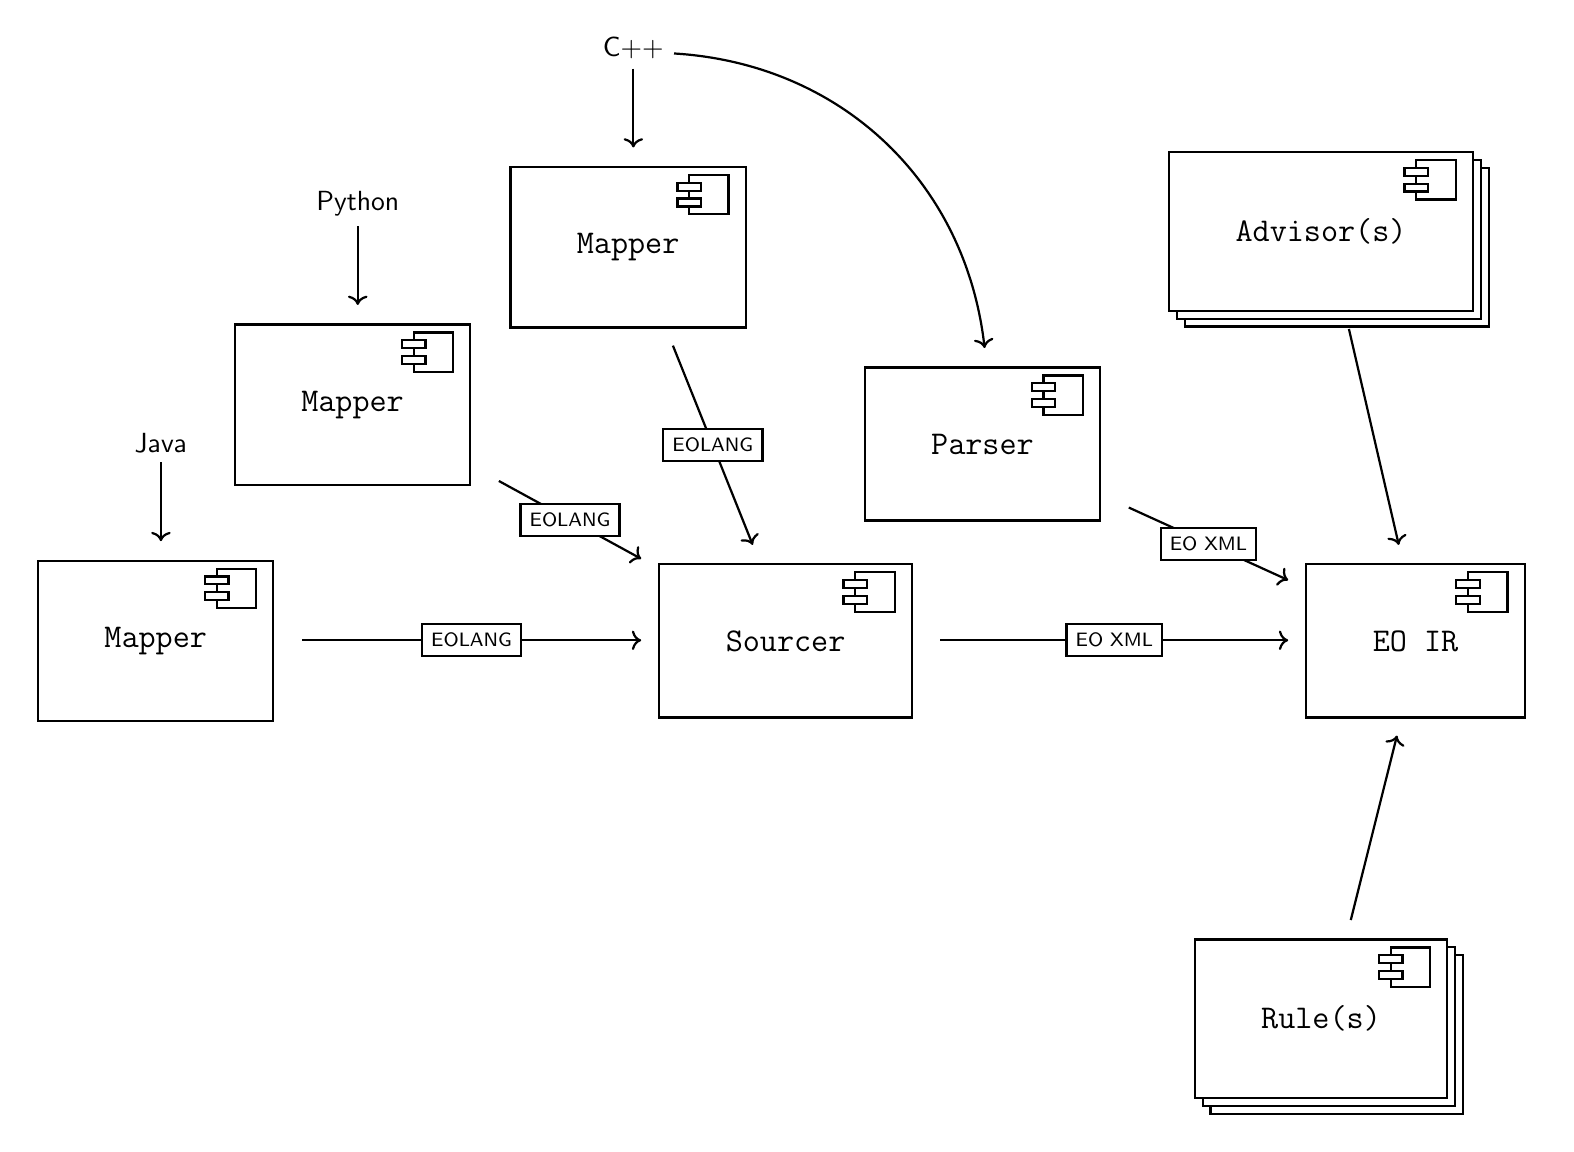
\begin{tikzpicture}
  \component{ir}{6,5}{EO IR}
  \component{sourcer}{-2,5}{Sourcer}
  \component{java2eo}{-10,5}{Mapper}
  \component{python2eo}{-7.5,8}{Mapper}
  \component{cpp2eo}{-4,10}{Mapper}
  \component{advisors1}{5,10}{Advisor(s)}
    \component{advisors2}{4.9,10.1}{Advisor(s)}
    \component{advisors}{4.8,10.2}{Advisor(s)}
  \component{rules1}{5,0}{Rule(s)}
    \component{rules2}{4.9,0.1}{Rule(s)}
    \component{rules}{4.8,0.2}{Rule(s)}
  \component{parser}{0.5,7.5}{Parser}

  \node [above=1cm of java2eo] (java) {Java};
  \draw[->] (java) edge (java2eo);

  \node [above=1cm of cpp2eo] (cpp) {C++};
  \draw[->] (cpp) edge (cpp2eo);

  \node [above=1cm of python2eo] (python) {Python};
  \draw[->] (python) edge (python2eo);

  \draw[->] (cpp) to[bend left=40] (parser);
  \draw[->] (parser) edge node {EO XML} (ir);

  \draw[->] (cpp2eo) edge node {EOLANG} (sourcer);
  \draw[->] (java2eo) edge node {EOLANG} (sourcer);
  \draw[->] (python2eo) edge node {EOLANG} (sourcer);
  \draw[->] (sourcer) edge node {EO XML} (ir);
  \draw[->] (rules) edge (ir);
  \draw[->] (advisors) edge (ir);
\end{tikzpicture}};
\caption{UML Component Diagram of key elements wired together}
\label{fig:architecture}
\end{figure}

\section{Expected Outcomes}

\sector{Scientific Effect}
If the suggested research plan succeeds, the following positive outcome is possible
for computer science and the domain of programming languages in particular:
\begin{itemize}
  \item OOP will finally obtain its lacking component---object calculus;
  \item It will help design better languages, compilers, and static analyzers;
  \item New and better methods of static analysis will be introduced.
\end{itemize}

\sector{Industry Effect}
The industry of software development may benefit too:
\begin{itemize}
  \item The quality of software will be increased, meaning
  less functional bugs (there are many other quality aspects of
  software to be increased, but this one is the most obvious and
  measurable);
  \item New programming language may become an alternative to Java and C++;
  \item It may be used in \nospell{microservices}, embedded software, and so on;
  \item New polyglot static analyzer may outperform CSA
  with better soundness and accuracy by at least 10\%,
  as mentioned in the Section~\ref{sec:evaluation};
  \item The maintainability and security of the source code written
  by millions of programmers may be improved through the introduction
  of a common formal ground of OOP;
  \item The analyzer may be open-sourced and certified to help software teams
  deliver higher quality of code with no additional costs.
\end{itemize}

\sector{Probability of Success}
Even though, as was demonstrated above, many attempts to formalize
object-oriented programming were not successful, we believe that
our new research may produce the outcome we are looking for.
First, as Section~\ref{sec:prior} explained, our existing
tools, libraries, and frameworks empirically demonstrated the solidness
of the new paradigm.
Second, modern higher-level programming languages like Kotlin and Groovy,
are much further away from low-level procedural paradigm, which dominated
when first attempts to formalize OOP were made---this situation gives us higher
chances to succeed.
Third, the first version of our new object calculus has already been created
and a new programming language on top it was implemented---this proof-of-concept,
if future research is done properly, is a promising indicator of success.

\PrintBibliography

\end{document}
